
\documentclass{standalone}

\begin{document}
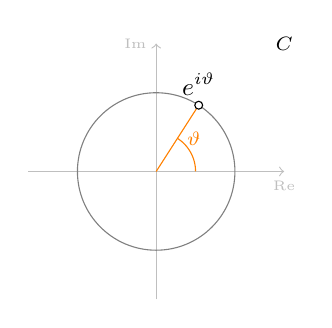
\begin{tikzpicture}
\usetikzlibrary{decorations.pathreplacing,angles,quotes}
\usetikzlibrary{shapes.geometric,shapes.misc}
\usetikzlibrary{calc}

\def\GRIDSIZE{1.625}
\draw[lightgray,->] (0, -\GRIDSIZE) -- (0, \GRIDSIZE)
    node[left] {\tiny Im};
\draw[lightgray,->] (-\GRIDSIZE, 0) -- (\GRIDSIZE, 0)
    node[below] {\tiny Re};
\draw (\GRIDSIZE, \GRIDSIZE) node {\scriptsize $\mathbb C$};

\draw[gray] (0, 0) circle (1);

\def\TH{1.0}

\def\R{0.5}
\draw[orange,domain=0:\TH]
    plot ({\R*cos(deg(\x))}, {\R*sin(deg(\x))})
    node[right] {\scriptsize $\vartheta$};

\coordinate (P) at ({cos(deg(\TH))}, {sin(deg(\TH))});
\draw[orange] (0, 0) -- (P);
\draw[fill=white] (P) circle (.05)
    node[above] {\small $e^{i \vartheta}$};


\end{tikzpicture}
\end{document}
